\section{Identifying continuous time systems using impulse and step response}
In this section we will consider an example of a linear time invariant continuous time system and see how we can use the provided toolbox as well as built in Matlab functions to identify the system.

\subsection{Defining the system}
We will be considering a simple mass damper spring system with the following state space representation.

\begin{figure}[H]
	\centering
	
\includegraphics[width=0.3\textwidth]{MSD.png}
	\caption{Free body diagram of mass damper spring system.}
\end{figure}

\begin{equation*}
\begin{bmatrix}
\dot{x} \\ \ddot{x}
\end{bmatrix} = 
\begin{bmatrix}
0 & 1 \\ \frac{-k}{M} & \frac{-f_v}{M}
\end{bmatrix}  
\begin{bmatrix}
x \\ \dot{x}
\end{bmatrix} +
\begin{bmatrix}
0 \\ \frac{1}{M}
\end{bmatrix} 
u
\end{equation*}

In this example we will assume that the mass, damping coefficient and spring coefficient are $1$. We will define this system in Matlab as follows.

\begin{lstlisting}
A = [0 1 ; -1 -1];
B = [0 ; 1];
C = eye(2);
D = [];
sys_c = ss(A,B,C,D);
\end{lstlisting}

Before we consider the data we will make a note about a condition that we need on our input. We will note that we assume our input to be constant between samples, i.e. we assume our input to be constant or a step function with discontinuities at the measurement intervals. This will ensure that we can uniquely map our continuous time system to a discrete time system using the zero order hold transform \cite{kollar1996equivalence}. 

We will be considering both the data generated by the impulse response as well as the step response. These will ensure that the assumption on the input signal is satisfied.

\subsection{Impulse response}
We will start by generating data using the Matlab function \mon{[y, t, x] = impulse(sys)}.

\begin{lstlisting}
[~, t, x] = impulse(sys_c);
\end{lstlisting}

\begin{figure}[H]
	\centering
	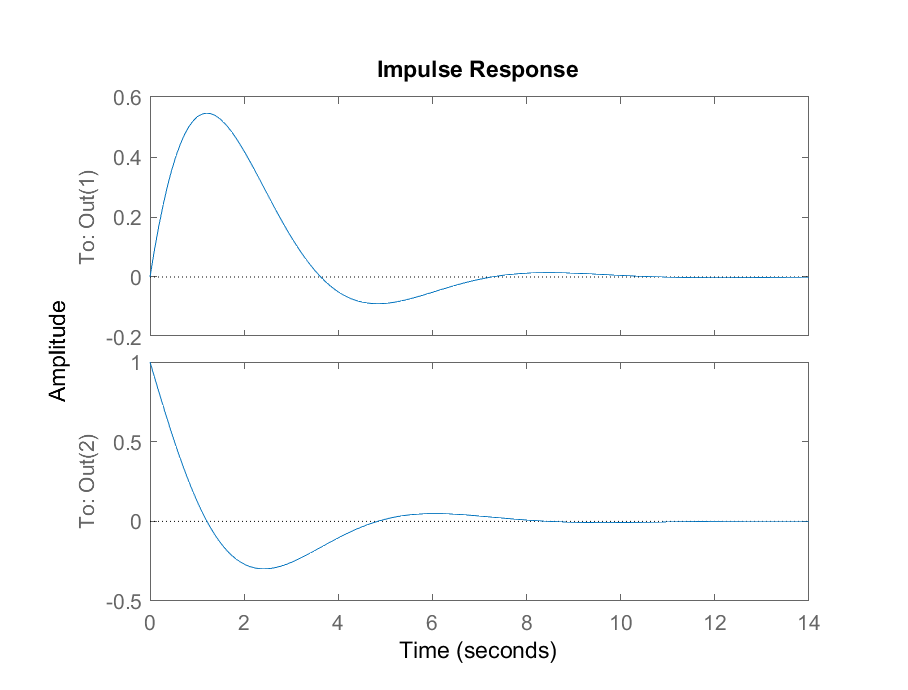
\includegraphics[width=0.7\textwidth]{impulse_response_msd.eps}
	\caption{Impulse response plot of the mass damper spring system.}
\end{figure}

Since we are considering the impulse responce of the system, we know that the input will be constant zero. Hence we will consider the system to be unforced for the time being. We will use the data to reconstruct the $A$ matrix of the system.

In the case of system identification we need that the matrix containing both $X_-$ and $U_-$ is full rank. Since our input data is constant zero we will not be able to identify the discrete time system matrices $A_d$ and $B_d$. However, due to our input being zero we are able to consider the system as if it had no input and hence we are able to identify the descrete time $A_d$ matrix. Note that for our state data to be compatible with the function from the toolbox we need to transpose is to be a wide matrix instead of a tall one.

\begin{lstlisting}
x = x';
[bool, A_d] = isInformIdentification(x)
\end{lstlisting}

Which will return that the data is indeed informative for system identification and gives us the following discrete time $A_d$ matrix.

\begin{equation*}
	A_d = \begin{bmatrix}
		 0.9959 &   0.0879 \\
		-0.0879 &   0.9080
	\end{bmatrix}
\end{equation*}

Now we need to verify that the continuous time counterpart of this descrete time $A_d$ matrix is indeed the same as our original system. For this we will use the function \mon{sysc = d2c(sysd)} provided by matlab to transform a discrete time system to a continuous time system. Note that we need to define a time step for our discrete time system, we can retreive the time step from the \mon{t} matrix returned by the impulse responce function.

\begin{lstlisting}
sys_d = ss(A_d, [], [], [], t(2));
A_c = d2c(sys_d).A
\end{lstlisting}

This will return the following continuous time $A_c$ matrix.

\begin{equation*}
	A_c = \begin{bmatrix}
		-0.0000 &   1.0000\\
		-1.0000 &  -1.0000
	\end{bmatrix}
\end{equation*}

As we can see our computed $A_c$ matrix is almost the same as the true $A$ matrix. The larges difference as computed by matlab between entries of the matrices is $0.3e-14$ which makes them the same up to machine precision.

\subsection{Step response}
We will now be considering the step responce of the system. We will pick our input to be constant $1$. Using this we will repeat the previous steps to see if we are able to accuratly recover both the $A$ and $B$ system matrices. We will generate the data using the built in Matlab function \mon{[y, t, x] = step(sys)}. 

\begin{lstlisting}
[~, t, x] = step(sys_c);
\end{lstlisting}

\begin{figure}[H]
	\centering
	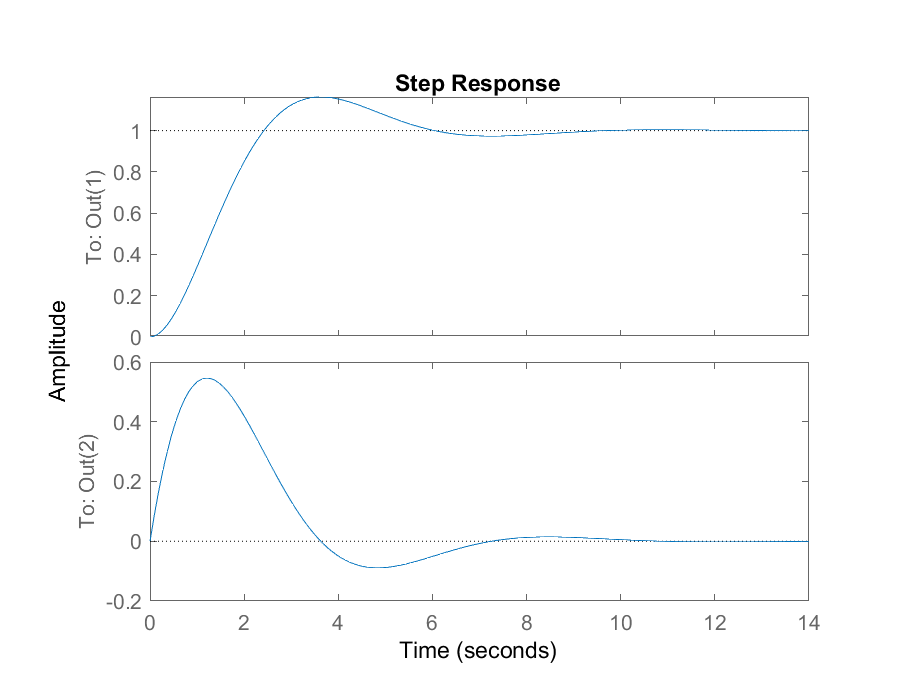
\includegraphics[width=0.7\textwidth]{step_response_msd.eps}
	\caption{Step response plot of the mass damper spring system.}
\end{figure}

Since our input data is non zero it might be the case that the matrix containing both $X_-$ and $U_-$ is full rank. Before we check if the data is informative for system identification we will prepare the data to be used for the toolbox.

\begin{lstlisting}
x = x';
U = ones(1,size(x,2) - 1);
[bool, A_d, B_d] = isInformIdentification(x, U)
\end{lstlisting}

From this we can indeed see that the data is informative for system identification and that the discrete time system matrices are given as:

\begin{align*}
	A_d &= \begin{bmatrix} 0.9959 & 0.0879 \\ -0.0879 & 0.9080 \end{bmatrix} &
	B_d &= \begin{bmatrix} 0.0041 \\ 0.0879 \end{bmatrix} 
\end{align*}

We will once again convert these to a continuous time system using \mon{sysc = d2c(sysd)} with the time step as defined in the \mon{t} matrix returned by the step function.

\begin{lstlisting}
sys_d = ss(A_d, B_d, [], [], t(2));
A_c = d2c(sys_d).A
B_c = d2c(sys_d).B
\end{lstlisting}

Which will return the following continuous time system matrices.

\begin{align*}
A_d &= \begin{bmatrix} 0.0000 & 1.0000 \\ -1.0000 & -1.0000 \end{bmatrix} &
B_d &= \begin{bmatrix} 0.0000 \\ 1.0000 \end{bmatrix} 
\end{align*}

As we can see the computed continuous time system matrices are again the same as the true system up to machine presision.
